\beginsong{Un bravo lupo}

\begin{tikzpicture}[remember picture, overlay]
    \node[inner sep=0pt, anchor=south east] 
    at ([yshift=0.7cm]current page text area.south east) { % Centra l'immagine nella pagina
        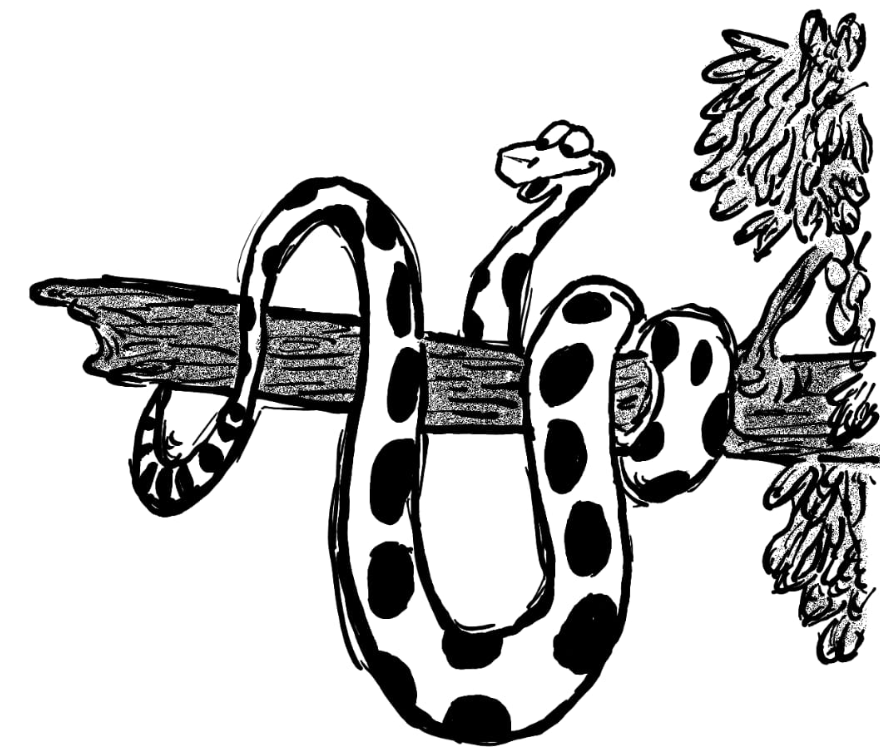
\includegraphics[width=0.45\paperwidth]{img/kaa.png} 
    };
\end{tikzpicture}

\begin{tikzpicture}[remember picture, overlay]
    \node[opacity=0.15,inner sep=0pt, anchor=center, rotate=90, xscale=-1, yscale=-1] 
    at ([xshift=-2cm,yshift=2cm]current page text area.center) {
        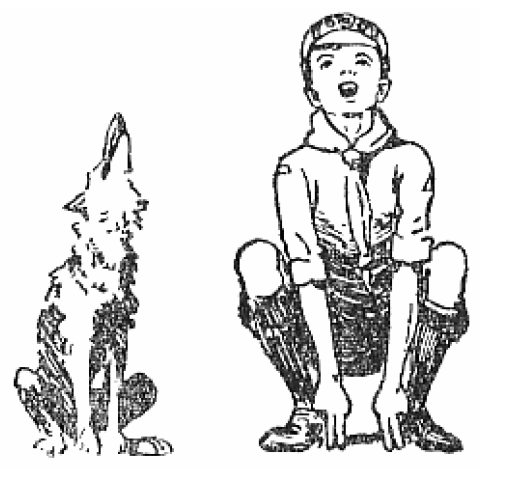
\includegraphics[width=0.8\paperwidth]{img/ulula.png} 
    };
\end{tikzpicture}

\beginchorus
    \[LA]Un bravo lupo io \[RE]voglio diventar \\
    \[MI]E la promessa per \[LA]sempre rispettar \\
    Gentile e più cor\[LA7]tese con tut\[RE]ti io sarò\\
    la buona a\[MI]zion\\
    sempre \[LA]farò
\endchorus

\beginverse
    Akela \[MI]oh, Akela \[LA]oh te lo promet\[MI]to, più in \[MI7]gamba io sa\[LA]rò \rep{2}\\
\endverse

\chordsoff

\beginverse
    Caro Baloo, caro Baloo\\
    io la Legge osserverò di più \rep{2}
\endverse

\beginverse
    Bagheera oh, Bagheera oh\\
    te lo prometto in caccia io verrò \rep{2}
\endverse

\beginverse
    Mio caro Kaa, mio caro Kaa\\
    te lo prometto, farò tante B.A. \rep{2}
\endverse

\beginverse
    Mio caro Chil, mio caro Chil\\
    te lo prometto, sarò sempre gentil \rep{2}
\endverse
\endsong